%%%%%%%%%%%%%%%%%%%%%%%%%%%%%%%%%%%%%%%%%%%%%%%%%%%%%%%%%%%%%%%%%%%%%%%%%%
%                                                                        %
%                            INTRODUCTION                                %
%                                                                        %
%%%%%%%%%%%%%%%%%%%%%%%%%%%%%%%%%%%%%%%%%%%%%%%%%%%%%%%%%%%%%%%%%%%%%%%%%%
\subsection*{}
%%%%%%%%%%%%%%%%%%%%%%%%%%%%%%%%%%%%%%%%%%%%%%%%%%%%%%%%%%%%%%%%%%%%%%%%%%
\begin{frame}{Neutron - Gamma Discrimination}
  \begin{columns}[onlytextwidth]
    \begin{column}{0.45\textwidth}
    \large
    Methods of Neutron - Gamma Discrimination
    \normalsize
    \begin{itemize}
      \item Pulse shape 
      \item Pulse height
      \item Limit interactions
    \end{itemize}
    \end{column}
    \begin{column}{0.45\textwidth}
      How thick does a detector need to be to have less than one in a million interactions?
      \vspace{1cm}
      \begin{align*}
        \num{1E-6} &\le 1-\exp\left ( \frac{-\mu}{\rho}t \right )  
      \end{align*}
      \pause
      \huge
      \textcolor{red}{160 nm}
    \end{column}
  \end{columns}
\end{frame}
%%%%%%%%%%%%%%%%%%%%%%%%%%%%%%%%%%%%%%%%%%%%%%%%%%%%%%%%%%%%%%%%%%%%%%%%%%
\begin{frame}[t]{Pulse Height Discrimination}
\label{PHDMain}
  \begin{itemize}
    \item Use a lower lever discriminator to discard counts
    \item Mathematical Lower Lever Discriminator (MLLD)
  \end{itemize}
  \begin{columns}[onlytextwidth]
    \begin{column}{0.7\textwidth}
      \begin{figure}
          \vspace*{-1cm}
          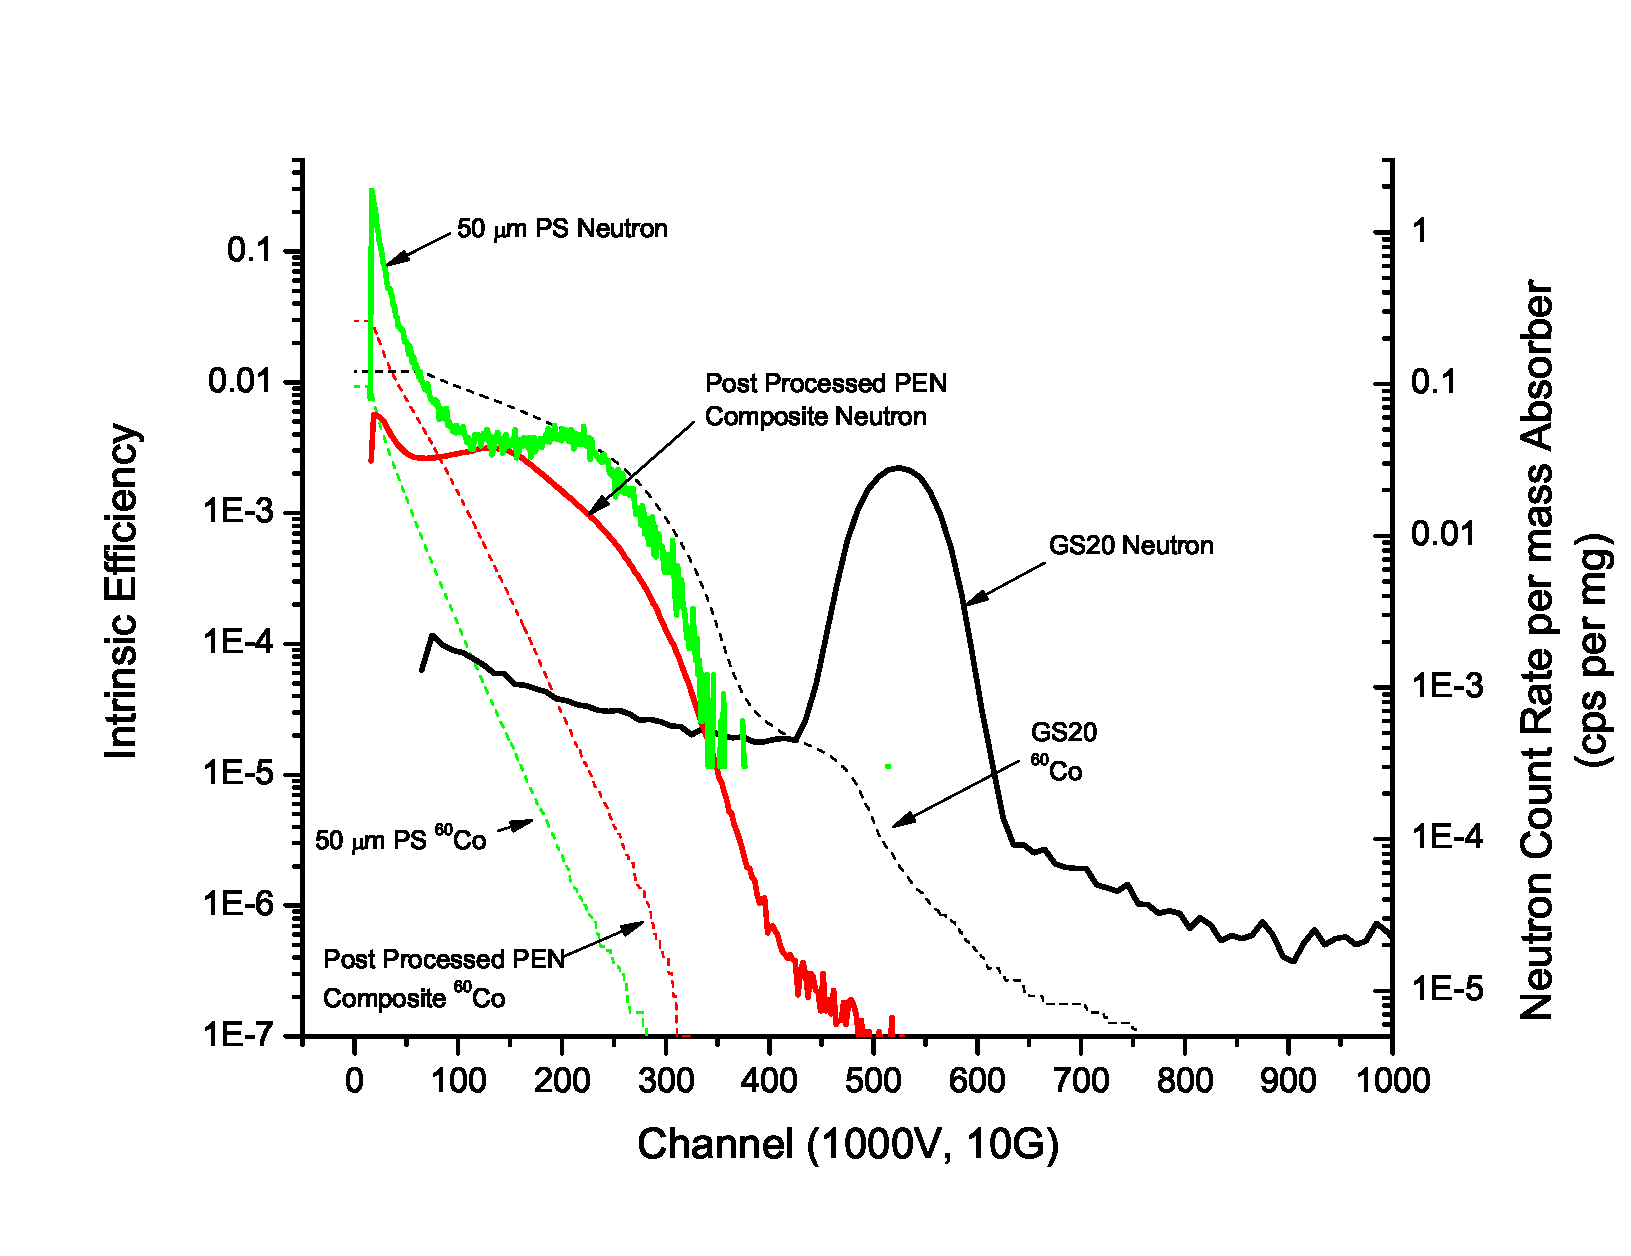
\includegraphics[width=\textwidth]{SC_UTDetectors_IntEff_CR}
      \end{figure}
    \end{column}
    \begin{column}{0.25\textwidth}
  \begin{align*}
    \frac{dL}{dx} = \frac{S_B\frac{dE}{dx}}{1+kB\frac{dE}{dx}}
  \end{align*}
    \end{column}
  \end{columns}
  Pulse height discrimination is equivalent to the energy deposition
\hyperlink{MeasMethods}{\beamerbutton{Measurment Setups and Methods}}
\end{frame}
%%%%%%%%%%%%%%%%%%%%%%%%%%%%%%%%%%%%%%%%%%%%%%%%%%%%%%%%%%%%%%%%%%%%%%%%%%
